\documentclass[11pt,a4paper]{article}
\usepackage[utf8]{inputenc}
\usepackage[margin=22mm,top=18mm,bottom=18mm]{geometry}
\usepackage{amsmath,amssymb}
\usepackage{tikz}
\usetikzlibrary{shapes.geometric, arrows.meta, positioning}
\usepackage{titlesec}
\usepackage{caption}

% Section styling & spacing
\titlespacing*{\section}{0pt}{6pt plus 1pt minus 1pt}{3pt plus 1pt minus 1pt}
\titleformat{\section}{\large\bfseries}{\thesection}{0.6em}{}
\setlength{\parskip}{4pt}
\setlength{\parindent}{0pt}
\captionsetup{font=small,skip=4pt}

\title{\vspace{-8mm}\LARGE\textbf{Physics-Informed Machine Learning Vessel Depth Classification}}
\author{\large\textbf{Roy Michael} \\
\normalsize Department of Marine Technologies, Haifa University \\
\normalsize \textit{Breaking the Surface (BtS) 2026 Student Poster}}
\date{\vspace{-5mm}}

\begin{document}

\maketitle

\begin{abstract}
\normalsize
Passive acoustic depth classification in shallow maritime channels is challenged by non-stationary boundary interactions.
This work proposes a physics-informed classification framework distinguishing surface vessels from submerged acoustic sources.
Theoretical modeling reveals that surface vessels couple to ocean swell, causing heave-induced kinematic frequency modulation (FM) and dynamic micro-multipath interference (a doubly spread channel), resulting in characteristic spectral smearing.
Conversely, submerged sources decouple from surface dynamics, isolating multipath into additive, resolvable echoes and preserving sharp, unmodulated engine tonals.
By integrating time-series buffering, channel transfer parameter estimation, Doppler stability indicators, and bandwidth expansion metrics, our pipeline extracts physics-grounded features for robust, interpretable machine learning classification.
\end{abstract}

\vspace{2mm}

\section{Introduction}
Passive Acoustic Monitoring (PAM) is essential for maritime surveillance and autonomous robotic perception.
Discriminating surface craft from submerged platforms using acoustic signatures remains difficult because shallow ocean channels induce complex acoustic smearing governed by dynamic boundary scattering.
Purely data-driven classifiers often fail to generalize across varying sea states.
We address this by embedding analytical channel models, specifically heave-induced kinematic modulation and dynamic micro-multipath scattering directly into the classification pipeline.

\section{Theoretical Modeling of Acoustic Propagation}
\textbf{Surface-Coupled Sources (Doubly Spread Channel):} A surface vessel ($H_{src} \approx 0$) experiences vertical heave displacement $z(t) = A_w \sin(2\pi f_w t)$, phase-modulating the emitted tonal $p_0(t) = P_0 \cos(2\pi f_0 t)$ into an FM signal with modulation index $\beta = \frac{2\pi f_0}{c} A_w \cos\theta_g$.
By Jacobi-Anger expansion, this generates an infinite Bessel-weighted comb:
\begin{equation}
p_{tx}(t) = P_0 \sum_{n=-\infty}^{\infty} J_n(\beta) \cos\left(2\pi (f_0 + n f_w)t\right)
\end{equation}
At long ranges ($R \gg H_{rec}$), grazing angle $\theta_g \to 0^\circ$, causing direct and surface paths to overlap ($\Delta\tau \approx 0$). The total field experiences multiplicative, time-varying amplitude fading and dynamic Doppler phase spreading:
\begin{equation}
p_{rx}(t) \propto p_{tx}(t-\tau_{dir})\left[ 1 - R_0 \exp\left( i \frac{4\pi f_0}{c} h_s(t) \sin\theta_g \right) \right]
\end{equation}

\textbf{Submerged Sources (Decoupled Propagation):} Operating below the wave base ($H_{src} \gg 0$) eliminates vertical heave ($A_w \approx 0 \implies \beta \approx 0$). The Bessel comb collapses to a pure single tone ($J_0(0)=1$, $J_{n\neq 0}=0$). Furthermore, path length differences become macroscopic ($R_{surf} \gg R_{dir}$), temporally isolating the surface reflection ($\Delta\tau \gg 0$) into an additive, resolvable echo:
\begin{equation}
p_{rx}(t) = \frac{P_0}{R_{dir}}\cos\left(2\pi f_0 (t-\tau_{dir})\right) + \frac{P_0 V(t)}{R_{surf}}\cos\left(2\pi f_0 (t-\tau_{surf})\right)
\end{equation}
leaving the primary direct-path arrival sharp, narrowband, and temporally stable.

\begin{figure}[h!]
\centering
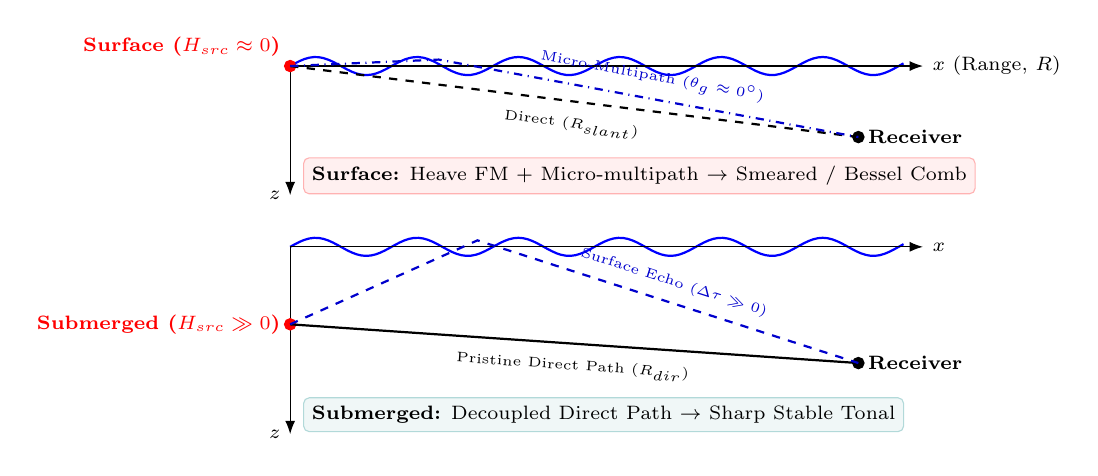
\begin{tikzpicture}[scale=0.82, >=Latex]
    % Surface
    \draw[thick, blue, domain=0:9.5, samples=130] plot (\x, {3.2 + 0.14*sin(4*\x r)});
    \draw[->, thin] (0,3.2) -- (9.8,3.2) node[right, font=\scriptsize] {$x$ (Range, $R$)};
    \draw[->, thin] (0,3.2) -- (0,1.2) node[left, font=\scriptsize] {$z$};
    \filldraw[red] (0,3.2) circle (2.5pt) node[above left, font=\scriptsize, text=red] {\textbf{Surface ($H_{src}\approx 0$)}};
    \filldraw[black] (8.8,2.1) circle (2.5pt) node[right, font=\scriptsize] {\textbf{Receiver}};
    \draw[dashed, thick] (0,3.2) -- (8.8,2.1) node[midway, below=2pt, sloped, font=\tiny] {Direct ($R_{slant}$)};
    \draw[dashdotted, thick, blue!80!black] (0,3.2) -- (2.3,3.3) -- (8.8,2.1) node[midway, above=1pt, sloped, font=\tiny] {Micro-Multipath ($\theta_g \approx 0^\circ$)};
    \node[anchor=west, fill=red!6, draw=red!30, rounded corners=2pt, inner sep=3pt, font=\scriptsize] at (0.2, 1.5) {\textbf{Surface:} Heave FM + Micro-multipath $\rightarrow$ Smeared / Bessel Comb};

    % Submerged
    \begin{scope}[yshift=-2.8cm]
        \draw[thick, blue, domain=0:9.5, samples=130] plot (\x, {3.2 + 0.14*sin(4*\x r)});
        \draw[->, thin] (0,3.2) -- (9.8,3.2) node[right, font=\scriptsize] {$x$};
        \draw[->, thin] (0,3.2) -- (0,0.3) node[left, font=\scriptsize] {$z$};
        \filldraw[red] (0,2.0) circle (2.5pt) node[left, font=\scriptsize, text=red] {\textbf{Submerged ($H_{src} \gg 0$)}};
        \filldraw[black] (8.8,1.4) circle (2.5pt) node[right, font=\scriptsize] {\textbf{Receiver}};
        \draw[thick] (0,2.0) -- (8.8,1.4) node[midway, below=2pt, sloped, font=\tiny] {Pristine Direct Path ($R_{dir}$)};
        \draw[dashed, thick, blue!80!black] (0,2.0) -- (2.9,3.3) -- (8.8,1.4) node[midway, above=1pt, sloped, font=\tiny] {Surface Echo ($\Delta\tau \gg 0$)};
        \node[anchor=west, fill=teal!6, draw=teal!30, rounded corners=2pt, inner sep=3pt, font=\scriptsize] at (0.2, 0.6) {\textbf{Submerged:} Decoupled Direct Path $\rightarrow$ Sharp Stable Tonal};
    \end{scope}
\end{tikzpicture}
\caption{Propagation physics: surface-coupled scattering vs. submerged decoupling.}
\label{fig:propagation}
\end{figure}

\section{Generalized Signal Processing \& Classification Pipeline}
The end-to-end framework maps the physical channel behaviors into a compact, discriminative machine learning feature space via a generalized four-stage pipeline (Fig.~\ref{fig:pipeline}).

\begin{figure}[h!]
\centering
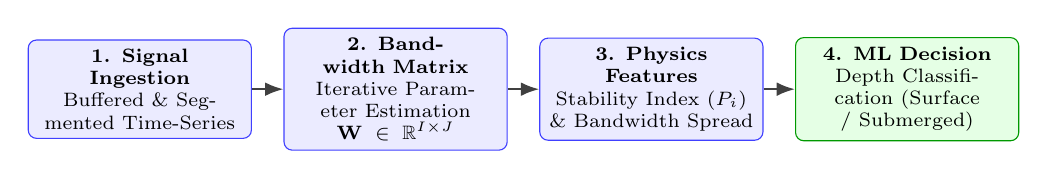
\begin{tikzpicture}[
    node distance=0.4cm,
    block/.style={rectangle, draw=blue!75, fill=blue!8, text width=2.6cm, text centered, rounded corners=3pt, minimum height=1.0cm, font=\scriptsize},
    arrow/.style={-Latex, thick, draw=black!75}
]
    \node (s1) [block] {\textbf{1. Signal Ingestion}\\Buffered \& Segmented Time-Series};
    \node (s2) [block, right=of s1] {\textbf{2. Bandwidth Matrix}\\Iterative Parameter Estimation $\mathbf{W} \in \mathbb{R}^{I \times J}$};
    \node (s3) [block, right=of s2] {\textbf{3. Physics Features}\\Stability Index ($P_i$) \& Bandwidth Spread};
    \node (s4) [block, fill=green!10, draw=green!60!black, right=of s3] {\textbf{4. ML Decision}\\Depth Classification (Surface / Submerged)};

    \draw [arrow] (s1) -- (s2);
    \draw [arrow] (s2) -- (s3);
    \draw [arrow] (s3) -- (s4);
\end{tikzpicture}
\caption{Generalized physics-informed classification architecture.}
\label{fig:pipeline}
\end{figure}

\begin{enumerate}
    \setlength{\itemsep}{2pt}
    \item \textbf{Signal Ingestion:} Raw hydrophone data is buffered into $J$ temporal windows (1-second analysis frames).
    \item \textbf{Bandwidth Parameter Matrix:} For $I$ candidate spectral frequencies $f_{c,i}$, instantaneous bandwidth and transmission responses are compiled into matrix $\mathbf{W} \in \mathbb{R}^{I \times J}$.
    \item \textbf{Physics-Informed Feature Extraction:}
    \begin{itemize}
        \setlength{\itemsep}{1pt}
        \item \textit{Stability Indicator ($P_i$):} Tracks temporal variance in signal envelopes to detect destructive micro-multipath fading.
        \item \textit{Bandwidth Expansion Metric:} Quantifies spectral broadening.
    \end{itemize}
    \item \textbf{Machine Learning Decision Engine:} Extracted features are fed into a lightweight decision-making classifier to deliver real-time depth classification.
\end{enumerate}

\section{Conclusion \& Work-in-Progress}
By incorporating ocean wave kinematics and boundary scattering physics directly into feature extraction, this architecture prevents overfitting and enhances generalization across diverse sea states.
Current work focuses on validating the pipeline on experimental shallow-water acoustic datasets for real-time detection of autonomous underwater vehicles (AUVs) and diver propulsion vehicles (DPVs).

\end{document}